\documentclass{article}

\usepackage[utf8]{inputenc}
\usepackage[margin=1in]{geometry}
\usepackage{amsmath, amssymb, xcolor, polynom}
\usepackage{amsfonts}
\usepackage{hyperref}
\usepackage{enumitem}
\usepackage{multirow}
\usepackage{tikz}
\usetikzlibrary{automata,shapes,shapes.geometric,arrows,fit,calc,positioning}
 
\begin{document}

\pagenumbering{gobble}

\begin{titlepage}

\newcommand{\HRule}{\rule{\linewidth}{0.5mm}}

\center

\textsc{\huge University of Waterloo}\\[2cm]
\textsc{\LARGE SE465}\\[1cm] 
\textsc{\Large Section 001}\\[1cm] 

\HRule \\[0.5cm]
{ \Huge \bfseries Project}\\[0.5cm] 
\HRule \\[0.5cm]
 
\LARGE Zhoatian \textsc{Fang} \\  [0.5cm]
\Large 20519284 \\  [0.5cm]
z23fang@uwaterloo.ca \\ [1.5cm]

\LARGE Andrew \textsc{Zhou} \\  [0.5cm]
\Large 20509626 \\  [0.5cm]
a25zhou@uwaterloo.ca \\ [1.5cm]

\LARGE Di Sen \textsc{Lu} \\  [0.5cm]
\Large 20519284 \\  [0.5cm]
z23fang@uwaterloo.ca \\ [1.5cm]

{\Large \today}\\

\vfill 

\end{titlepage}

\section*{Part (I) Building an Automated Bug Detection Tool}

\subsection*{(b) Finding and Explaining False Positives}
Let's assume that there's high confidence and support for the pair of functions A and B such that A and B are often included as pairs of function calls. In other words, most of the time, all callers of function A will also call function B and vice versa. \\

One fundamental reason for why false positives occur is when A is called by a function but B is not also called by the function. Instead, the functions calls a ``caller'' of B, which will in turn call B. This will throw a bug in the root function because it finds a call to A but no matching call to B. However, this bug is a false positive since the root function does call B, but it does so by first calling a ``caller'' of B, and then the function B itself. \\
To illustrate this false positive scenario, after examining the output of our program for (a) on the Apache \verb|httpd| server, we found that the pair of functions \verb|(apr_array_make,apr_array_push| often occur together. 
For some background context, the use of the function \verb|apr_array_make| is simply to allocate enough space to create an empty array \\
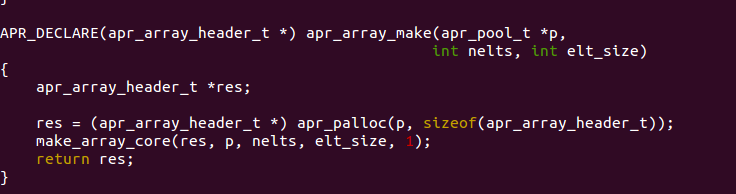
\includegraphics[scale=0.5]{ss/apr_array_make_def.png} \\
Its pairing function, \verb|apr_array_push| is used to resize/recreate the array in the scenario that amount of elements used in the array is nearing the array's capacity. \\
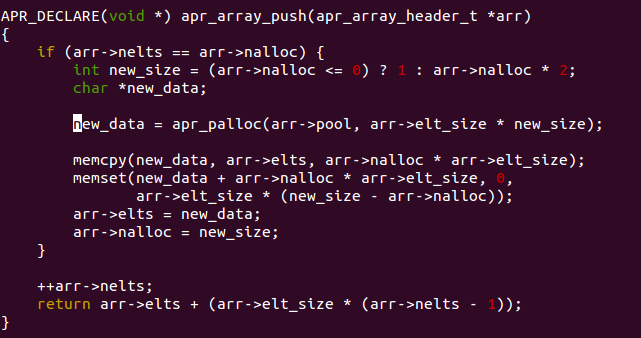
\includegraphics[scale=0.5]{ss/apr_array_push_def.png} \\
Therefore, it is intuitive that these functions should be paired together in the scenario where you populate an array with a variable number of data elements, so you'll have to create the array and constantly resize it depending on how many elements need to be added. \\
From the output, we found 10 lines where \verb|apr_array_push| is called but \verb|apr_array_make| isn't. \\
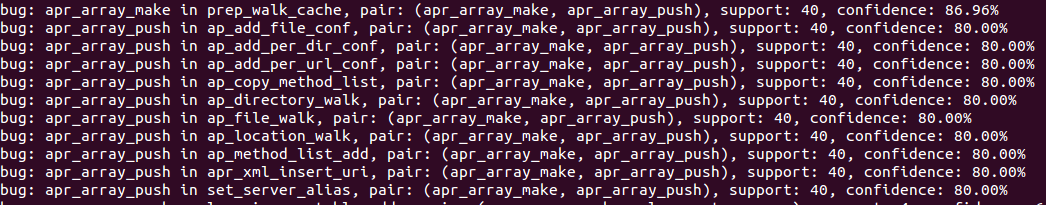
\includegraphics[scale=0.5]{ss/apr_array_push_false_positives.png}
In particular, we'll examine the case where the root function is \verb|ap_location_walk|. Inside the function definition for \verb|ap_location_walk|, we can see that \verb|ap_array_push| is indeed called. \\
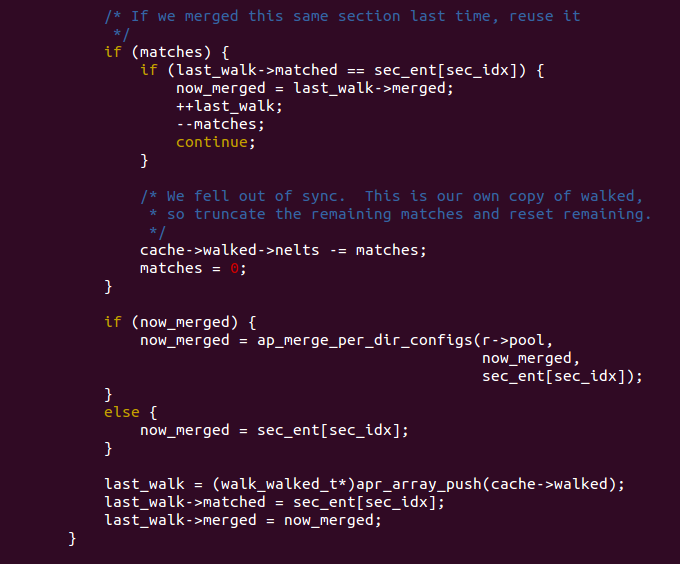
\includegraphics[scale=0.5]{ss/unravel_one_level_proof3.png} \\
However, we could not find any matching calls to \verb|apr_array_make|! After some closer inspection, we found that \verb|ap_location_walk| calls \verb|prep_walk_cache|. \\
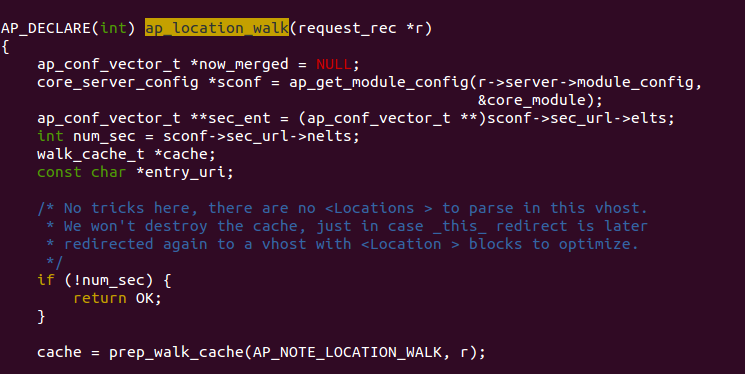
\includegraphics[scale=0.5]{ss/unravel_one_deep_proof2.png} \\
Inside the function definition, we find that \verb|prep_walk_cache| is the function that calls \verb|apr_array_make|! \\
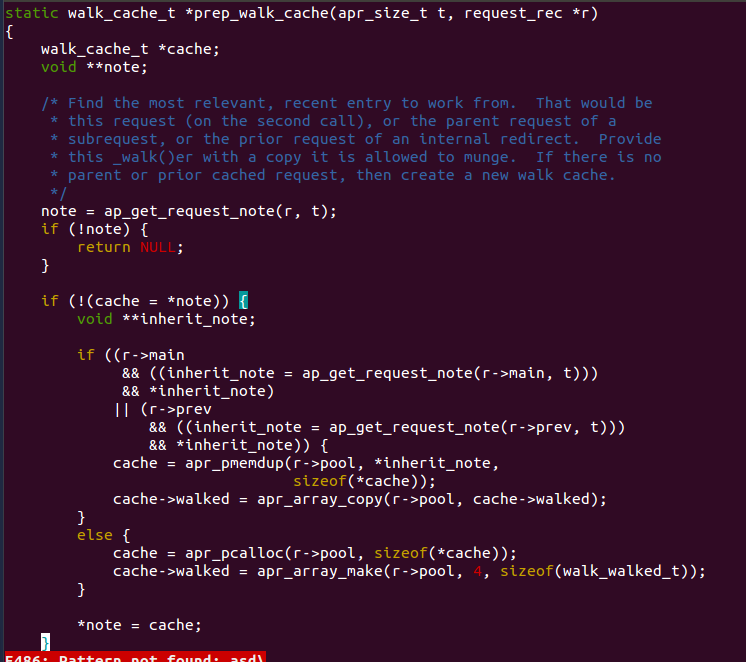
\includegraphics[scale=0.5]{ss/unravel_one_level_proof.png} \\
Therefore, the reason that the false positive occured is because \verb|ap_location_walk| calls \verb|ap_array_push| but not \verb|ap_array_make|. However, this bug is not correct since \verb|ap_location_walk| does call \verb|ap_array_make|, but indirectly by first calling \verb|prep_walk_cache| and then \verb|ap_array_make|. \\

Another fundamental reason for why false positives occur is when A and B are two functions that do \textbf{need} to be called together, but are often called together because their functions complement each other in helping to accomplish a common task. \\
To illustrate this fundamental reason, we took a look at the pair of functions \verb|(ms_release_conn,strlen)| that are often called together. For a bit of background on the two functions, \verb|ms_release_conn| performs some cleanup operations when closing/finishing a socket connection. The \verb|strlen| function simply returns the length of a string based on the number of characters it contains. \\
After examining the bug output, we found 3 lines where \verb|ms_release_conn| is called but \verb|strlen| isn't. \\
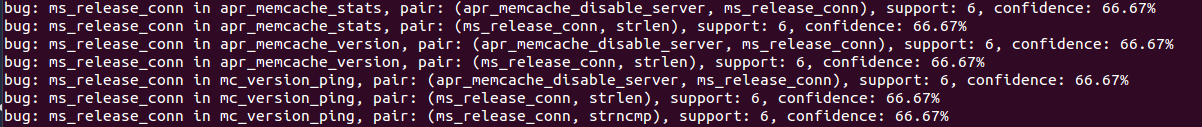
\includegraphics[scale=0.5]{ss/ms_release_conn_strlen_false_positives.png} \\
In particular, we'll look at the instance where the caller of the pair of functions is \verb|mc_version_ping|. The definition of the function is shown below \\
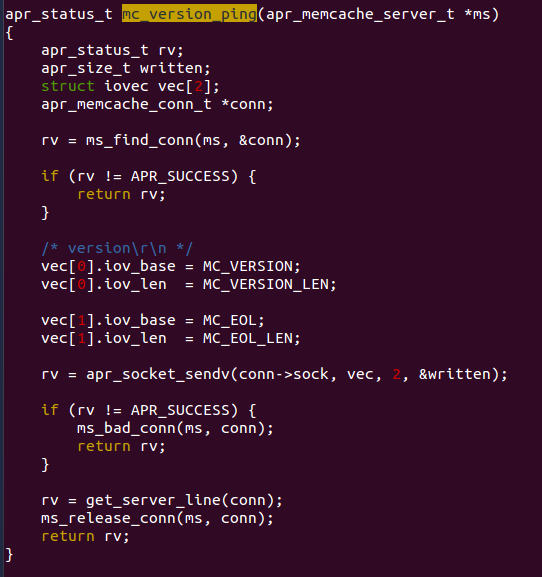
\includegraphics[scale=0.5]{ss/release_conn_no_strlen.png} \\
The use of this function is simply to create a socket connection to a server, ping it with a message, and then return the response as a string from the server. It is true that \verb|ms_release_conn| is called but \verb|strlen| isn't, but more analysis needs to be done to determine why these pair of functions have a strong support in the first place. The function \verb|mget_conn_result| uses both \verb|ms_release_conn| and \verb|strlen|. The function definition is shown below \\
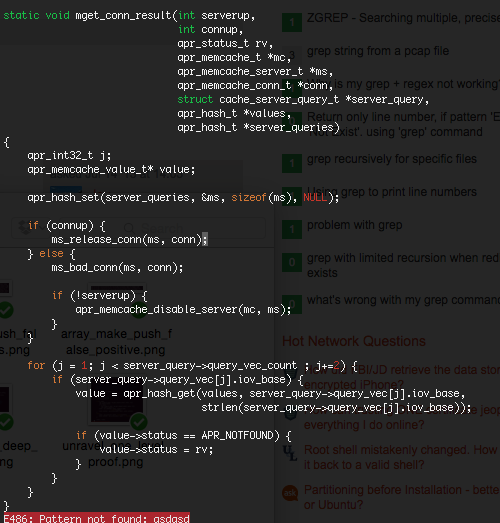
\includegraphics[scale=0.5]{ss/ms_release_conn_strlen_usage.png} \\
The use of the two functions in this scenario is to first close the connection if it is still open using \verb|ms_release_conn|, and then using the data retrieved from the socket connection, update the \verb|apr_hash| hash table. The use of \verb|strlen| is simply to pass the length of the key to a hash table operator function. Using this information it is clear why the bug in \verb|mc_version_ping| is a false positive. For other functions where \verb|ms_release_conn| is called, it often needs to perform hash table updates using data retrieved from the socket connection. The hash table updates needs to know about the length of the key, which is why \verb|strlen| is often called too. In the case of the function \verb|mc_version_ping|, it creates a socket connection, but it doesn't do any hash table operations using the data retrieved from the socket connection, so it makes sense that \verb|strlen| is not called.

\subsection*{(c) Inter-Procedural Analysis}

\section*{Part (II) --- Using a Static Bug Detection Tool}

\subsection*{(a) Resolving Bugs in Apache Commons}
\begin{itemize}
\item \textbf{CID 10065: Bug} \\
    Lines 639-640, filename: /src/java/org/apache/commons/lang/BooleanUtils.java \\
    The case should return false if the first character isn't y, but instead falls through to the next case.
    Could be a problem with a three letter string that starts with y and isn't yes. \\
    \textbf{Proposed fix:} Add an $else { return false; }$ statement at line 639.
\item \textbf{CID 10066: Bug} \\
    Line 70, filename: /src/java/org/apache/commons/lang/text/StrBuilder.java \\
    StrBuilder class doesn't implement/override Object.clone() method. Bad practice - either do not make
    StrBuilder implement Cloneable, or provide an actual clone() method, otherwise users trying to clone
    StrBuilder may be unable to succeed. \\
    \textbf{Proposed fix:} Override and implement a proper Object.clone() method, or stop StrBuilder from 
    implementing Cloneable.
\item \textbf{CID 10067: False Positive} \\
    Line 292, filename: /src/java/org/apache/commons/lang/exception/NestableDelegate.java \\
    We believe that the encoding to be used for printStackTrace(PrintStream out) is inherently the user's responsibility because
    the PrintStream object determines what charset to use. As such, it should be fine to use the default encoding of the out object.
\item \textbf{CID 10068: Intentional} \\
    Line 110, filename: /src/java/org/apache/commons/lang/math/JVMRandom.java \\
    The choice to use Math.random() seems intentional due to the docstring mentioning the use of the Math.random() sequence.
    The code can be refactored by using $Random.nextInt(n)$ instead of $((int)Math.random() * n)$, which provides a performance
    boost on average (see: \url{http://community.oracle.com/message/6596485}).
\item \textbf{CID 10069: Intentional} \\
    Line 552, filename: /src/java/org/apache/commons/lang/enum/Enum.java \\
    The docstring for equals() specifies that the desired behaviour for testing equality is to ensure that the class names and 
    object names are equal. Checking class names for equality is a bad practice because malicious users can provide non-equivalent
    classes with the same name (see: \url{http://cwe.mitre.org/data/definitions/486.html}). However, because a class object equality 
    check is done prior to this check, we have already safeguarded for this possibility, so this method of comparison can be left in as-is.
\item \textbf{CID 10070: Intentional} \\
    Line 598, filename: /src/java/org/apache/commons/lang/enums/Enum.java \\
    Duplicate of \textbf{CID 10069}, please see above.
\item \textbf{CID 10071: Bug} \\
    Line 614, filename: /src/java/org/apache/commons/lang/BooleanUtils.java \\
    Use of object reference equality comparison operator $==$ instead of the $.equals()$ method leads to undesired behaviour if for example
    a String object created explicitly by the $new \enspace String()$ constructor is passed in instead of a string literal. If $new \enspace String(''true'')$
    is passed in rather than $''true''$, then the comparison will return false when we want it to return true. \\
    \textbf{Proposed fix:} Use $''true''.equals(str)$ instead on line 614.
\item \textbf{CID 10072: Bug} \\
    Line 4865, filename: /src/java/org/apache/commons/lang/StringUtils.java \\
    Like with \textbf{CID 10071}, use of the object reference equality comparison operator $==$ instead of the .equals() method will not work 
    for String objects that are not simply literals (ie. those created explicitly by a String constructor). \\
    \textbf{Proposed fix:} Replace lines 4865-4870 with the following: first check for (str1 == null $\Vert$ str2 == null), which is the check on line 4868.
    Return 0 if this is true. Then, check that str1.equals(str2), and return -1 if that is true.
\item \textbf{CID 10073: Bug} \\
    Lines 385-409, filename: /src/java/org/apache/commons/lang/time/DurationFormatUtils.java \\
    Like with \textbf{CID 10071} and \textbf{CID 10072}, should use .equals() method instead. \\
    \textbf{Proposed fix:} Replace instances of == with value.equals().
\item \textbf{CID 10074: Bug} \\
    Line 485, filename: /src/java/org/apache/commons/lang/time/DurationFormatUtils.java \\
    Same as above. \\
    \textbf{Proposed fix:} Replace previous.getValue() == value with previous.getValue().equals(value).
\item \textbf{CID 10075: Bug} \\
    Line 649, filename: /src/java/org/apache/commons/lang/Entities.java \\
    If the array is sufficiently large and the key being searched for has a sufficiently high index, it is possible to get an integer
    overflow from the calculation of (low + high), which is clearly undesired behaviour. \\
    \textbf{Proposed fix:} Change the algorithm for calculating mid. Replace line 649 with: int mid = low + (high - low) / 2
\item \textbf{CID 10076: False Positive} \\
    Line 64, filename: /src/java/org/apache/commons/lang/BooleanUtils.java \\
    The desired behaviour of this method as indicated by the docstring is to return null when a null value is passed in.
    There is value in having the possibility of a Boolean being null, instead of true or false 
    (see: \url{http://stackoverflow.com/questions/11185321/when-should-null-values-of-boolean-be-used}), so we believe that
    if a null object is passed into the negate() function, there is an explicit reason for this and that we should not
    modify the value into either true or false as this does not make semantic sense.
\item \textbf{CID 10077: False Positive} \\
    Line 313, filename: /src/java/org/apache/commons/lang/BooleanUtils.java \\
    Like \textbf{CID 10076}, there is semantic value in returning a null value for a Boolean, and this method's docstring
    explicitly states that its intended behaviour is to return a null value if the given value input matches the given nullValue input.
\item \textbf{CID 10078: False Positive} \\
    Line 225, filename: /src/java/org/apache/commons/lang/BooleanUtils.java \\
    Like \textbf{CID 10076} and \textbf{CID 10077}, a null Boolean has a distinct meaning separate from true and false, and 
    so the intended behaviour of this method returning null if a null Integer is passed in can make sense and is not 
    necessarily a bad practice.
\item \textbf{CID 10079: False Positive} \\
    Lines 345 and 352, filename: /src/java/org/apache/commons/lang/BooleanUtils.java \\
    Very similar to \textbf{CID 10077}, the methods share the behaviour of potentially returning a null Boolean object
    at the discretion of the user's input, and it remains that having a null Boolean object can provide utility that
    returning true or false would not provide, so this method's behaviour seems acceptable.
\item \textbf{CID 10080: False Positive} \\
    Line 538, filename: /src/java/org/apache/commons/lang/BooleanUtils.java \\
    Arguably, it might make sense to return true or false instead if the string does not match true, false, 
    on, off, yes, or no. However, returning null also makes sense as it means that the string does not represent
    any boolean concept and so has no boolean value.
\item \textbf{CID 10081: False Positive} \\
    Lines 567 and 574, filename: /src/java/org/apache/commons/lang/BooleanUtils.java \\
    Duplicate of \textbf{CID 10077} and \textbf{CID 10079}.
\item \textbf{CID 10082: Intentional} \\
    Line 97, filename: /src/java/org/apache/commons/lang/exception/ExceptionUtils.java \\
    Likely to be intentional by a developer as a means of lazily catch-alling any exception and setting the causeMethod
    to null regardless of the exception, it is still bad practice to ignore the exception thrown by getMethod(). Although
    leaving the code as-is is unlikely to be too harmful, it is advised that the catch statements be more fine-grained so that 
    runtime exceptions can be caught and logged for future debugging.
\item \textbf{CID 10083: Bug} \\
    Line 137, filename: /src/java/org/apache/commons/lang/time/FastDateFormat.java \\
    Potentially an oversight, the field mRules is not serializable and so it is bad practice to leave it 
    as is because the FastDateFormat class implements the Serializable interface. \\
    \textbf{Proposed fix:} Either the mRules field should be marked transient if the intent of the developers 
    is for the rules to be lost on serialization, or alternatively the readObject() and writeObject() methods 
    should be implemented to manually serialize mRules if the intent is to save this field's state upon serialization.
\item \textbf{CID 10084: False Positive} \\
    Line 84, filename: /src/java/org/apache/commons/lang/IntHashMap.java \\
    The field hash is read by methods such as containsKey(key), get(key), etc., which are all public methods of
    IntHashMap defined later in the same Java file. As such, the field is used and the warning can be ignored.
\end{itemize}

\subsection*{(b) Analyzing Your Own Code}
After running Coverity on our program from part (I) (a), it has detected two defects in our code. \\
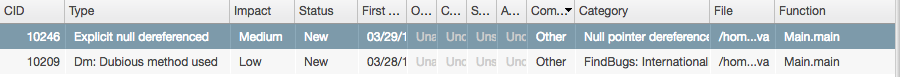
\includegraphics[scale=0.5]{ss/coverity_bugs.png} \\

The first defect deals dereferencing a variable \verb|curNode|, which could be null at the time of its usage. \\
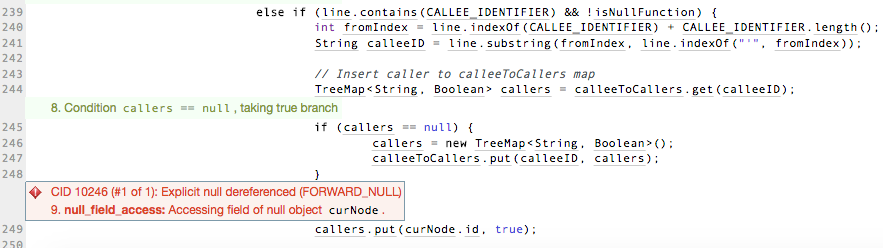
\includegraphics[scale=0.5]{ss/bug_null_dereference.png} \\
The use of the variable \verb|curNode| is to store the current caller function so we can add its callees to the \verb|curNode| variable as we're parsing the callgraph. The defect can be fixed by simply adding a null-check before we add a function as \verb|curNode|'s callee. However, when we were coding it, we made the assumption that \verb|curNode| should always be non-null before we add callees to it. This is generally true based on the structure of the callgraph. \\
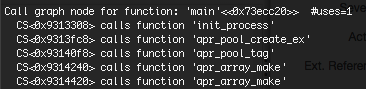
\includegraphics[scale=0.5]{ss/example_callgraph.png} \\
Based on a typical callgraph that we see above, its true that during callgraph parsing, we'll always read a line like ``Call graph node for function: $<$function$\_$name$>$...'' that initialized \verb|curNode| with the current caller function before we read lines like ``CS$<$mem$\_$addr$>$ calls function $<$callee$\_$function$\_$name$>$'' which adds callees to the caller function. Therefore, the program should never crash due to omitting the null check but it should be there anyways in case the callgraph format ever changes and for proper programming practice. \\

The second defect deals with our use of the class \verb|Scanner|, which reads the callgraph passed to the graph line by line. \\
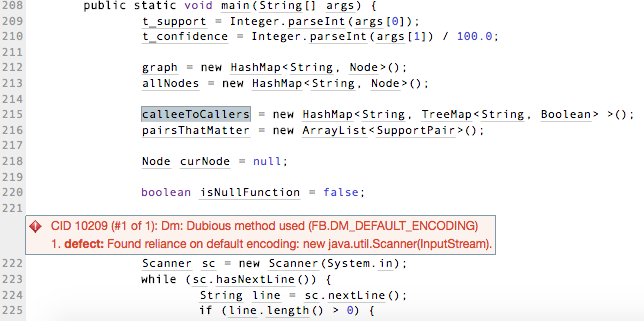
\includegraphics[scale=0.5]{ss/bug_dubious_method.png} \\

\end{document}
